% answers.tex —— 1988 年·广东卷·理工农医类 · 参考答案与详细解析片段
% 由 tools/generate_projects.py 依来源总账自 1988/1988_数学真题_广东理_试题.md + 1988/1988_数学真题_广东理_解析正文.md + 1988/1988_数学真题_广东理_答案要点.md 生成，勿手改（改源 MD 后重跑）


\begin{gktip}
固定源 PDF 第 5—9 页含答案与解答。以下按题号规范化转录并统一数学记号；第 1 题第（23）小题的题面图形在固定源中缺失，因此只能记录固定源答案表的 A，不能据现有 PDF 独立核验。
\end{gktip}

\begin{answer}
\gksolhead{1}{}

\textbf{题目}：

第一卷满分 50 分，共有 25 个选择题。每题都给出代号为 A、B、C、D 的四个结论，其中只有一个结论正确。每题选对得 2 分，不选、选错或者选出的代号超过一个，一律得 0 分。

（1） 直线 $3x-2y=6$ 在 $y$ 轴上的截距是\mbox{（　　）}

（A）$\dfrac32$　　（B）$-2$　　（C）$-3$　　（D）$3$

\Needspace{5\baselineskip}
（2） 对数方程

\nopagebreak[4]
\[
2\log_6x=1-\log_6 3
\]

的解是\mbox{（　　）}

（A）$\sqrt3$　　（B）$\sqrt2$　　（C）$\sqrt2$ 和 $-\sqrt2$　　（D）$\sqrt3$ 和 $\sqrt2$

（3） 如果用 $C\text{、}R$ 和 $I$ 分别表示复数集、实数集和纯虚数集，其中 $C$ 为全集，那么有\mbox{（　　）}

（A）$C=R\cup I$　　（B）$R\cap I=\{0\}$

（C）$\overline R=C\cap I$　　（D）$R\cap I=\varnothing$

（4） 在等差数列 $\{a_n\}$ 中，已知前 15 项之和 $S_{15}=90$，那么 $a_8=$\mbox{（　　）}

（A）$3$　　（B）$4$　　（C）$6$　　（D）$12$

（5） 如果 $\operatorname{tg}A+\operatorname{ctg}A=m$，那么 $\sin2A=$\mbox{（　　）}

（A）$\dfrac1m$　　（B）$\dfrac2m$　　（C）$2m$　　（D）$\dfrac1{m^2}$

（6） 设 $a\text{、}b$ 是异面直线，那么\mbox{（　　）}

（A）必然存在唯一的一个平面同时平行于直线 $a$ 和 $b$

（B）必然存在唯一的一个平面同时垂直于直线 $a$ 和 $b$

（C）过直线 $a$ 存在唯一的一个平面平行于直线 $b$

（D）过直线 $a$ 存在唯一的一个平面垂直于直线 $b$

\Needspace{5\baselineskip}
（7） 当 $a\ne0$ 时，方程

\nopagebreak[4]
\[
x^2+y^2+ax-ay=0
\]

所表示的图形\mbox{（　　）}

（A）关于 $x$ 轴对称　　（B）关于 $y$ 轴对称

（C）关于直线 $y-x=0$ 对称　　（D）关于直线 $y+x=0$ 对称

\Needspace{5\baselineskip}
（8） 设 $\theta$ 是第四象限的角，那么方程

\nopagebreak[4]
\[
(\sin\theta)x^2+y^2=\sin2\theta
\]

所表示的曲线是\mbox{（　　）}

（A）焦点在 $x$ 轴上的椭圆　　（B）焦点在 $y$ 轴上的椭圆

（C）焦点在 $x$ 轴上的双曲线　　（D）焦点在 $y$ 轴上的双曲线

\Needspace{5\baselineskip}
（9） 抛物线

\nopagebreak[4]
\[
y^2=4x-2
\]

的准线的方程是\mbox{（　　）}

（A）$x=-\dfrac12$　　（B）$x=\dfrac14$　　（C）$x=0$　　（D）$x=-1$

（10） 过抛物线 $y^2=4x$ 的焦点，作直线与此抛物线相交于两点 $P$ 和 $Q$，那么线段 $PQ$ 中点的轨迹的方程是\mbox{（　　）}

（A）$y^2=2x-1$　　（B）$y^2=2x-2$　　（C）$y^2=-2x+1$　　（D）$y^2=-2x+2$

（11） 设正方体的全面积为 $24\,\mathrm{cm}^2$，一个球内切于该正方体，那么，这个球的体积是\mbox{（　　）}

（A）$\dfrac43\pi\,\mathrm{cm}^3$　　（B）$\dfrac83\pi\,\mathrm{cm}^3$

（C）$\sqrt6\pi\,\mathrm{cm}^3$　　（D）$\dfrac{32}3\pi\,\mathrm{cm}^3$

（12） “平面 $\alpha$ 内有无穷多条直线都和直线 $l$ 平行”是“$l\parallel\alpha$”的\mbox{（　　）}

（A）充分而不必要的条件　　（B）必要而不充分的条件

（C）必要且充分的条件　　（D）既不充分又不必要的条件

（13） 下列函数中，在区间 $(0,1)$ 上是增函数的只有\mbox{（　　）}

（A）$y=-\sqrt{x}$　　（B）$y=\dfrac1{x^3}$　　（C）$y=\log_{\frac12}x$　　（D）$y=-x^2+2x+1$

\Needspace{5\baselineskip}
（14） 下列不等式中，与不等式

\nopagebreak[4]
\[
\frac{x-3}{2-x}\geq0
\]

同解的是\mbox{（　　）}

（A）$(x-3)(2-x)\geq0$　　（B）$\lg(x-2)\leq0$

（C）$\dfrac{2-x}{x-3}\geq0$　　（D）$(x-3)(2-x)>0$

（15） 用 $0\text{、}1\text{、}2\text{、}3\text{、}4$ 这五个数字组成没有重复数字的四位数，那么，在这些四位数中，是偶数的总共有\mbox{（　　）}

（A）120 个　　（B）96 个　　（C）60 个　　（D）36 个

\Needspace{5\baselineskip}
（16） 如果

\nopagebreak[4]
\[
\operatorname{tg}(\alpha+\beta)=\frac25,
\qquad \operatorname{tg}\left(\beta-\frac\pi4\right)=\frac14,
\]

\Needspace{5\baselineskip}
那么

\nopagebreak[4]
\[
\operatorname{tg}\left(\alpha+\frac\pi4\right)=
\]

\mbox{（　　）}

（A）$\dfrac{13}{18}$　　（B）$\dfrac{13}{22}$　　（C）$\dfrac3{22}$　　（D）$\dfrac3{18}$

（17） 函数值 $\operatorname{tg}224^\circ\text{、}\sin136^\circ\text{、}\cos310^\circ$ 的大小关系是\mbox{（　　）}

（A）$\operatorname{tg}224^\circ<\sin136^\circ<\cos310^\circ$

（B）$\sin136^\circ<\cos310^\circ<\operatorname{tg}224^\circ$

（C）$\cos310^\circ<\operatorname{tg}224^\circ<\sin136^\circ$

（D）$\cos310^\circ<\sin136^\circ<\operatorname{tg}224^\circ$

（18） 如果椭圆的两个焦点将长轴分成三等分，那么这个椭圆的两条准线间的距离是焦距的\mbox{（　　）}

（A）18 倍　　（B）12 倍　　（C）9 倍　　（D）4 倍

（19） 记函数 $y=\dfrac1x$ 的图象为 $l_1$，$y=\operatorname{arctg} x$ 的图象为 $l_2$，那么 $l_1$ 与 $l_2$ 的交点个数是\mbox{（　　）}

（A）无穷多个　　（B）2 个　　（C）1 个　　（D）0 个

（20） 如果实数 $x\text{、}y$ 满足 $x^2+y^2=1$，那么 $(1-xy)(1+xy)$ 有\mbox{（　　）}

（A）最小值 $\dfrac12$ 和最大值 1　　（B）最大值 1 和最小值 $\dfrac34$

（C）最小值 $\dfrac34$ 而无最大值　　（D）最大值 1 而无最小值

\Needspace{5\baselineskip}
（21） 曲线

\nopagebreak[4]
\[
y=1+\sqrt{4-x^2}\qquad(-2\leq x\leq2)
\]

与直线 $y=k(x-2)+4$ 有两个交点时，实数 $k$ 的取值范围是\mbox{（　　）}

（A）$\left(\dfrac5{12},\dfrac34\right]$　　（B）$\left(\dfrac5{12},+\infty\right)$

（C）$\left(\dfrac13,\dfrac34\right]$　　（D）$\left(0,\dfrac5{12}\right)$

\Needspace{5\baselineskip}
（22） 设 $f(x)$ 是 $R$ 上的奇函数，且当 $x\in[0,+\infty)$ 时，

\nopagebreak[4]
\[
f(x)=x(1+\sqrt[3]{x}),
\]

那么 $x\in(-\infty,0)$ 时，$f(x)=$\mbox{（　　）}

（A）$-x(1+\sqrt[3]{x})$　　（B）$x(1+\sqrt[3]{x})$

（C）$-x(1-\sqrt[3]{x})$　　（D）$x(1-\sqrt[3]{x})$

（23） 已知 $y=f(x)$ 的图象如右图，那么 $f(x)=$\mbox{（　　）}

\begin{gktip}
\textbf{转录疑点}：固定源题面明确写“如右图”，但固定 PDF 第 1—4 页中未见该图形；以下四个选项按可见文字转录，不凭空补图。
\end{gktip}

（A）$\sqrt{x^2-2|x|+1}$　　（B）$x^2-2|x|+1$

（C）$|x^2-1|$　　（D）$\sqrt{x^2-2x+1}$

\Needspace{5\baselineskip}
（24）　

\nopagebreak[4]
\[
\sqrt{1+\sin10}=
\]

\mbox{（　　）}

\begin{gktip}
\textbf{转录疑点}：固定源选项中的 $\sin10$、$\cos5$ 没有度数符号，按原卷字面记录。
\end{gktip}

（A）$\cos5+\sin5$　　（B）$-\cos5-\sin5$　　（C）$\sqrt2\cos5$　　（D）$\cos5-\sin5$

（25） 一个三棱锥，如果它的底面是直角三角形，那么它的三个侧面\mbox{（　　）}

（A）必然都是非直角三角形　　（B）至多只能有一个是直角三角形

（C）至多只能有两个是直角三角形　　（D）可能都是直角三角形

\Needspace{4\baselineskip}
\textbf{解析}

\gksubpart{（1）}

令 $x=0$，由 $3x-2y=6$ 得 $y=-3$，故选 C。

\gksubpart{（2）}

\Needspace{5\baselineskip}
由

\nopagebreak[4]
\[
2\log_6x=1-\log_6 3=\log_6 2
\]

得 $\log_6x^2=\log_6 2$。因 $x>0$，所以 $x=\sqrt2$，故选 B。

\gksubpart{（3）}

按本题“纯虚数”的约定，纯虚数不含实数 $0$，所以实数集与纯虚数集没有公共元素，即 $R\cap I=\varnothing$，故选 D。

\gksubpart{（4）}

\Needspace{5\baselineskip}
等差数列前 15 项的中项为第 8 项，故

\nopagebreak[4]
\[
S_{15}=15a_8=90,
\qquad a_8=6.
\]

故选 C。

\gksubpart{（5）}

\nopagebreak[4]
\[
\operatorname{tg}A+\operatorname{ctg}A
=\frac{\sin^2A+\cos^2A}{\sin A\cos A}
=\frac1{\sin A\cos A}=m.
\]

因此 $\sin2A=2\sin A\cos A=\dfrac2m$，故选 B。

\gksubpart{（6）}

过异面直线 $a$ 上一点作与直线 $b$ 平行的直线，该直线与 $a$ 确定唯一平面；该平面过 $a$ 且平行于 $b$。故选 C。

\gksubpart{（7）}

\Needspace{5\baselineskip}
配方得

\nopagebreak[4]
\[
\left(x+\frac a2\right)^2+\left(y-\frac a2\right)^2=\frac{a^2}{2}.
\]

圆心为 $\left(-\dfrac a2,\dfrac a2\right)$，在直线 $y=-x$ 上，故圆关于 $y+x=0$ 对称，选 D。

\gksubpart{（8）}

第四象限角满足 $\sin\theta<0$、$\sin2\theta<0$。方程两边同除以 $-\sin2\theta$ 后，二次项的符号相反，表示双曲线；含 $x^2$ 的系数为正，实轴在 $x$ 轴上，故选 C。

\gksubpart{（9）}

\nopagebreak[4]
\[
y^2=4x-2=4\left(x-\frac12\right).
\]

\Needspace{5\baselineskip}
这是顶点为 $\left(\dfrac12,0\right)$、参数 $p=1$ 的抛物线，准线为

\nopagebreak[4]
\[
x=\frac12-1=-\frac12\text{，}
\]

故选 A。

\gksubpart{（10）}

\Needspace{5\baselineskip}
抛物线焦点为 $(1,0)$。设过焦点的非竖直直线为 $y=t(x-1)$，与抛物线交于两点。若中点为 $(X,Y)$，代入并用韦达定理得

\nopagebreak[4]
\[
X=1+\frac2{t^2},qquad Y=\frac2t.
\]

消去 $t$，得到 $Y^2=2X-2$。竖直弦的中点 $(1,0)$ 也满足此式，故轨迹为 $y^2=2x-2$，选 B。

\gksubpart{（11）}

\Needspace{5\baselineskip}
设正方体棱长为 $s$，则 $6s^2=24$，所以 $s=2$。内切球半径为 $1$，体积为

\nopagebreak[4]
\[
\frac43\pi\cdot1^3=\frac43\pi\,\mathrm{cm}^3\text{，}
\]

故选 A。

\gksubpart{（12）}

若 $l\parallel\alpha$，则平面 $\alpha$ 内有无穷多条直线与 $l$ 平行，因此该条件是必要的。反之，若 $l$ 本身落在 $\alpha$ 内，则也可有无穷多条平行线，但不能按本题的“不相交平行”定义称为 $l\parallel\alpha$，故不是充分条件，选 B。

\gksubpart{（13）}

\Needspace{5\baselineskip}
在 $(0,1)$ 上，$-\sqrt x$、$x^{-3}$ 和 $\log_{1/2}x$ 均为减函数，而

\nopagebreak[4]
\[
\frac{d}{dx}(-x^2+2x+1)=2-2x>0.
\]

所以只有 D 为增函数，选 D。

\gksubpart{（14）}

\Needspace{5\baselineskip}
原不等式的解集为 $(2,3]$。又

\nopagebreak[4]
\[
\lg(x-2)\leq0
\Longleftrightarrow 0<x-2\leq1
\Longleftrightarrow 2<x\leq3\text{，}
\]

故选 B。

\gksubpart{（15）}

\Needspace{5\baselineskip}
末位为 $0$ 时，首位有 4 种、中间两位有 $3\cdot2$ 种，共 $24$ 个；末位为 $2$ 或 $4$ 时，每种有 $3\cdot3\cdot2=18$ 个。因此偶数共有

\nopagebreak[4]
\[
24+18+18=60\text{，}
\]

故选 C。

\gksubpart{（16）}

\Needspace{5\baselineskip}
由

\nopagebreak[4]
\[
\alpha+\frac\pi4=(\alpha+\beta)-\left(\beta-\frac\pi4\right)\text{，}
\]

\Needspace{5\baselineskip}
得

\nopagebreak[4]
\[
\operatorname{tg}\left(\alpha+\frac\pi4\right)
=\frac{\frac25-\frac14}{1+\frac25\cdot\frac14}
=\frac3{22}\text{，}
\]

故选 C。

\gksubpart{（17）}

\nopagebreak[4]
\[
\operatorname{tg}224^\circ=\operatorname{tg}44^\circ\text{，}
\qquad \sin136^\circ=\sin44^\circ\text{，}
\qquad \cos310^\circ=\cos50^\circ.
\]

显然 $\cos50^\circ<\sin44^\circ<\operatorname{tg}44^\circ$，故选 D。

\gksubpart{（18）}

设椭圆半长轴为 $a$、半焦距为 $c$。两个焦点把长轴分成三等分，所以 $a-c=2c$，即 $a=3c$，离心率 $e=c/a=1/3$。两准线距离为 $2a/e=6a$，焦距为 $2c=2a/3$，其比为 $9$，故选 C。

\gksubpart{（19）}

\Needspace{5\baselineskip}
交点横坐标满足

\nopagebreak[4]
\[
\frac1x=\operatorname{arctg} x\text{，}
\qquad x\operatorname{arctg} x=1.
\]

在 $x>0$ 上，$x\operatorname{arctg} x$ 从 $0$ 严格增至无穷，恰有一个根；该函数为偶函数，负半轴还有一个对称根，故共有 2 个交点，选 B。

\gksubpart{（20）}

\nopagebreak[4]
\[
(1-xy)(1+xy)=1-x^2y^2.
\]

由 $x^2+y^2=1$ 及 $2|xy|\leq x^2+y^2$，得 $|xy|\leq1/2$。故该式的最大值为 $1$，最小值为 $1-1/4=3/4$，选 B。

\gksubpart{（21）}

\Needspace{5\baselineskip}
曲线是圆心 $(0,1)$、半径 $2$ 的上半圆，直线恒过点 $(2,4)$。直线与圆相切的临界斜率由

\nopagebreak[4]
\[
\frac{|3-2k|}{\sqrt{k^2+1}}=2
\]

\Needspace{5\baselineskip}
得 $k=5/12$；直线经过左端点 $(-2,1)$ 时 $k=3/4$。要与上半圆有两个交点，故

\nopagebreak[4]
\[
\frac5{12}<k\leq\frac34\text{，}
\]

选 A。

\gksubpart{（22）}

\Needspace{5\baselineskip}
当 $x<0$ 时，令 $t=-x>0$。由奇函数性质

\nopagebreak[4]
\[
f(x)=-f(-x)=-t(1+\sqrt[3]{t})
=x(1-\sqrt[3]{x})\text{，}
\]

故选 D。

\gksubpart{（23）}

固定源题面所称“右图”在当前 PDF 中缺失，无法从图象排除选项。固定源答案表列为 A；本题保留该来源结论，并将图形缺失列入问题总账。

\gksubpart{（24）}

\Needspace{5\baselineskip}
恒有

\nopagebreak[4]
\[
1+\sin10=(\sin5+\cos5)^2.
\]

\Needspace{5\baselineskip}
因 $5$ 为弧度且 $\sin5+\cos5<0$，所以

\nopagebreak[4]
\[
\sqrt{1+\sin10}=|\sin5+\cos5|=-\cos5-\sin5\text{，}
\]

故选 B。固定源未给这两个数字加度数符号，按原卷解释为弧度。

\gksubpart{（25）}

底面为直角三角形并不能排除把顶点置于合适空间位置，使三个侧面分别在不同顶点处成为直角三角形；这种构造确实可能，因此“可能都是直角三角形”，选 D。

\gkanswer{答案（1）：C}

\gkanswer{答案（2）：B}

\gkanswer{答案（3）：D}

\gkanswer{答案（4）：C}

\gkanswer{答案（5）：B}

\gkanswer{答案（6）：C}

\gkanswer{答案（7）：D}

\gkanswer{答案（8）：C}

\gkanswer{答案（9）：A}

\gkanswer{答案（10）：B}

\gkanswer{答案（11）：A}

\gkanswer{答案（12）：B}

\gkanswer{答案（13）：D}

\gkanswer{答案（14）：B}

\gkanswer{答案（15）：C}

\gkanswer{答案（16）：C}

\gkanswer{答案（17）：D}

\gkanswer{答案（18）：C}

\gkanswer{答案（19）：B}

\gkanswer{答案（20）：B}

\gkanswer{答案（21）：A}

\gkanswer{答案（22）：D}

\gkanswer{答案（23）：A（固定源题面所称右图缺失，字母无法独立核验）}

\gkanswer{答案（24）：B}

\gkanswer{答案（25）：D}

\end{answer}
\begin{answer}
\gksolhead{2}{}

\textbf{题目}：

第二卷第一题（本题满分 15 分）共有 5 个小题，每小题满分 3 分。每个小题都有用横线表示的空位，请把你认为合适的内容写在横线上的空位里。

（1） 把极坐标方程 $\rho=4\sin\theta$ 化成直角坐标方程得　　　　。

（2） 函数 $y=|\cos x|$ 的最小正周期是　　　　。

（3） 复数 $-\sqrt6+\sqrt2i$ 的三角形式是　　　　。

\Needspace{5\baselineskip}
（4）　

\nopagebreak[4]
\[
\lim_{n\to\infty}
\frac{1-2+3-4+\cdots+(2n-1)-2n}{(n-1)\left(\frac1n+1\right)}
\]

的值是　　　　。

（5） 在 $(1+x+x^2)(1-x)^{10}$ 的展开式中，$x^5$ 的系数是　　　　。（用具体数字作答。）

\Needspace{4\baselineskip}
\textbf{解析}

\gksubpart{（1）}

\Needspace{5\baselineskip}
极坐标中 $x=\rho\cos\theta$、$y=\rho\sin\theta$。由 $\rho=4\sin\theta$ 得

\nopagebreak[4]
\[
\rho^2=4\rho\sin\theta=4y\text{，}
\]

\Needspace{5\baselineskip}
即

\nopagebreak[4]
\[
x^2+y^2-4y=0.
\]

\gksubpart{（2）}

因为 $|\cos(x+\pi)|=|{-\cos x}|=|\cos x|$，故最小正周期为 $\pi$。

\gksubpart{（3）}

\Needspace{5\baselineskip}
复数 $-\sqrt6+\sqrt2i$ 的模为 $2\sqrt2$，它位于第二象限，辐角为 $5\pi/6$，所以三角形式为

\nopagebreak[4]
\[
2\sqrt2\left(\cos\frac{5\pi}{6}+i\sin\frac{5\pi}{6}\right).
\]

\gksubpart{（4）}

\Needspace{5\baselineskip}
分子成对相减：

\nopagebreak[4]
\[
1-2+3-4+\cdots+(2n-1)-2n=-n.
\]

\Needspace{5\baselineskip}
分母为

\nopagebreak[4]
\[
(n-1)\left(1+\frac1n\right)=\frac{n^2-1}{n}\text{，}
\]

故极限为 $-1$。

\gksubpart{（5）}

\Needspace{5\baselineskip}
取 $x^5$ 项，来自 $1\cdot(1-x)^{10}$、$x\cdot(1-x)^{10}$ 和 $x^2\cdot(1-x)^{10}$ 中的相应项，系数为

\nopagebreak[4]
\[
(-1)^5\binom{10}{5}+(-1)^4\binom{10}{4}+(-1)^3\binom{10}{3}
=-252+210-120=-162.
\]

\gkanswer{答案（1）：$x^2+y^2-4y=0$}

\gkanswer{答案（2）：$\pi$}

\gkanswer{答案（3）：$2\sqrt2\left(\cos\dfrac{5\pi}{6}+i\sin\dfrac{5\pi}{6}\right)$}

\gkanswer{答案（4）：$-1$}

\gkanswer{答案（5）：$-162$}

\end{answer}
\begin{answer}
\gksolhead{3}{}

\textbf{题目}：

第二卷第二题（本题满分 13 分）。如图，在四棱锥 $P-ABCD$ 中，侧面 $PCD$ 是边长为 $2\,\mathrm{cm}$ 的等边三角形，且与底面垂直，而底面 $ABCD$ 是面积为 $2\sqrt3\,\mathrm{cm}^2$ 的菱形，$\angle ADC$ 是锐角。
\nopagebreak[4]
\begin{center}% 1988 年广东卷理工农医类第二卷第二题：四棱锥 P-ABCD
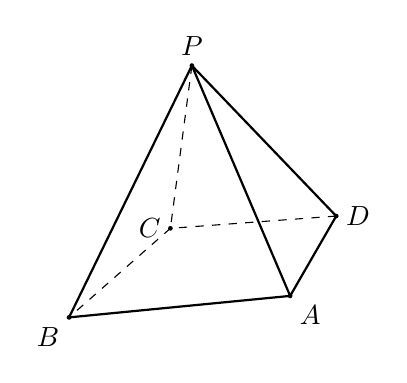
\begin{tikzpicture}[scale=0.78,>=stealth]
  \coordinate (P) at (2.0,4.1);
  \coordinate (B) at (0,0);
  \coordinate (A) at (3.6,0.35);
  \coordinate (D) at (4.35,1.65);
  \coordinate (C) at (1.65,1.45);
  \draw[thick] (P)--(B) (P)--(A) (P)--(D);
  \draw[dashed] (P)--(C);
  \draw[thick] (B)--(A)--(D);
  \draw[dashed] (D)--(C)--(B);
  \fill (P) circle (1.1pt) node[above] {$P$};
  \fill (A) circle (1.1pt) node[below right] {$A$};
  \fill (B) circle (1.1pt) node[below left] {$B$};
  \fill (C) circle (1.1pt) node[left] {$C$};
  \fill (D) circle (1.1pt) node[right] {$D$};
\end{tikzpicture}
\end{center}
\nopagebreak[4]
（1） 求这个四棱锥的体积。

（2） 求证：$PA\perp CD$。

\Needspace{4\baselineskip}
\textbf{解析}

\gksubpart{（1）}

\Needspace{5\baselineskip}
在等边三角形 $PCD$ 中作 $PE\perp CD$，则 $E$ 为 $CD$ 中点且 $PE=\sqrt3\,\mathrm{cm}$。侧面 $PCD$ 垂直于底面，故 $PE\perp$ 底面。于是四棱锥的高为 $PE$，体积

\nopagebreak[4]
\[
V=\frac13\cdot PE\cdot S_{ABCD}
=\frac13\cdot\sqrt3\cdot2\sqrt3=2\,\mathrm{cm}^3.
\]

\gksubpart{（2）}

\Needspace{5\baselineskip}
设 $\angle ADC=\theta$。菱形边长为 $2$，所以

\nopagebreak[4]
\[
2\sqrt3=S_{ABCD}=CD^2\sin\theta=4\sin\theta.
\]

因 $\theta$ 为锐角，得 $\theta=60^\circ$，从而底面三角形 $ADC$ 为等边三角形。$E$ 同时是 $CD$ 的中点，所以 $AE\perp CD$；又 $PE\perp CD$ 且 $AE\text{、}PE$ 相交于 $E$，故 $CD\perp$ 平面 $PAE$。因 $PA\subset$ 平面 $PAE$，得 $PA\perp CD$。

\gkanswer{答案（1）：$2\,\mathrm{cm}^3$}

\gkanswer{答案（2）：$PA\perp CD$}

\end{answer}
\begin{answer}
\gksolhead{4}{}

\textbf{题目}：

\Needspace{5\baselineskip}
第二卷第三题（本题满分 14 分）。已知双曲线的方程是

\nopagebreak[4]
\[
16x^2-9y^2=144.
\]

（1） 求这双曲线的焦点坐标、离心率和渐近线方程；

（2） 设 $F_1$ 和 $F_2$ 是这双曲线的左、右焦点，点 $P$ 在这双曲线上，且 $|PF_1|\cdot|PF_2|=32$，求 $\angle F_1PF_2$ 的大小。

\Needspace{4\baselineskip}
\textbf{解析}

\gksubpart{（1）}

\Needspace{5\baselineskip}
将方程化为标准式：

\nopagebreak[4]
\[
\frac{x^2}{3^2}-\frac{y^2}{4^2}=1.
\]

\Needspace{5\baselineskip}
故 $a=3$、$b=4$、$c=5$，焦点为 $F_1(-5,0)$、$F_2(5,0)$，离心率

\nopagebreak[4]
\[
e=\frac ca=\frac53\text{，}
\]

\Needspace{5\baselineskip}
渐近线为

\nopagebreak[4]
\[
y=\pm\frac ba x=\pm\frac43x.
\]

\gksubpart{（2）}

\Needspace{5\baselineskip}
令 $d_1=|PF_1|$、$d_2=|PF_2|$。双曲线的焦半径差满足 $|d_1-d_2|=2a=6$，而题设给出 $d_1d_2=32$。于是

\nopagebreak[4]
\[
d_1^2+d_2^2=(d_1-d_2)^2+2d_1d_2=36+64=100.
\]

\Needspace{5\baselineskip}
又 $|F_1F_2|=2c=10$，所以

\nopagebreak[4]
\[
|F_1F_2|^2=d_1^2+d_2^2.
\]

由勾股定理的逆定理，$\triangle F_1PF_2$ 在 $P$ 处为直角三角形，故 $\angle F_1PF_2=90^\circ$。

\gkanswer{答案（1）：焦点为 $F_1(-5,0)$、$F_2(5,0)$，离心率 $e=\dfrac53$，渐近线为 $y=\pm\dfrac43x$。}

\gkanswer{答案（2）：$\angle F_1PF_2=90^\circ$}

\end{answer}
\begin{answer}
\gksolhead{5}{}

\textbf{题目}：

\Needspace{5\baselineskip}
第二卷第四题（本题满分 14 分）。设 $0<\theta<2\pi$，复数

\nopagebreak[4]
\[
z=1-\cos\theta+i\sin\theta,qquad u=a^2+ai,
\]

且 $zu$ 是纯虚数，这里 $i$ 是虚数单位，$a$ 是实数。

（1） 求复数 $u$ 的辐角主值 $\arg u$（用 $\theta$ 的代数式表示）；

（2） 记 $\omega=z^2+u^2+2zu$，试问：$\omega$ 可能是正实数吗？为什么？

\Needspace{4\baselineskip}
\textbf{解析}

\gksubpart{（1）}

\Needspace{5\baselineskip}
设 $zu$ 为纯虚数，则其实部为零。直接相乘得

\nopagebreak[4]
\[
zu=\bigl[a^2(1-\cos\theta)-a\sin\theta\bigr]
+\bigl[a^2\sin\theta+a(1-\cos\theta)\bigr]i.
\]

\Needspace{5\baselineskip}
因此 $a\ne0$ 且

\nopagebreak[4]
\[
a(1-\cos\theta)=\sin\theta\text{，}
\qquad
a=\frac{\sin\theta}{1-\cos\theta}=\operatorname{ctg}\frac\theta2.
\]

\Needspace{5\baselineskip}
同时 $\theta\ne\pi$。由 $u=a^2+ai$ 得

\nopagebreak[4]
\[
\operatorname{tg}(\arg u)=\frac a{a^2}=\frac1a=\operatorname{tg}\frac\theta2.
\]

当 $0<\theta<\pi$ 时，$u$ 在第一象限，故 $\arg u=\theta/2$；当 $\pi<\theta<2\pi$ 时，$u$ 在第四象限，按 $[0,2\pi)$ 的主值约定，故 $\arg u=\pi+\theta/2$。

\gksubpart{（2）}

\Needspace{5\baselineskip}
有

\nopagebreak[4]
\[
\omega=z^2+u^2+2zu=(z+u)^2.
\]

\Needspace{5\baselineskip}
若 $\omega$ 为正实数，则 $z+u$ 必为实数，从而 $a+\sin\theta=0$，即 $a=-\sin\theta$。另一方面，由（1）有 $a=\sin\theta/(1-\cos\theta)$，且 $\sin\theta\ne0$。联立得到

\nopagebreak[4]
\[
-\sin\theta=\frac{\sin\theta}{1-\cos\theta}
\Longrightarrow \cos\theta=2\text{，}
\]

矛盾。因此 $\omega$ 不可能为正实数。

\gkanswer{答案（1）：当 $0<\theta<\pi$ 时，$\arg u=\dfrac\theta2$；当 $\pi<\theta<2\pi$ 时，$\arg u=\pi+\dfrac\theta2$。}

\gkanswer{答案（2）：不可能是正实数。}

\end{answer}
\begin{answer}
\gksolhead{6}{}

\textbf{题目}：

\Needspace{5\baselineskip}
第二卷第五题（本题满分 14 分）。设 $a>0$，$a\ne1$，

\nopagebreak[4]
\[
f(x)=\log_a\left(x+\sqrt{x^2-1}\right)\qquad(x\ge1).
\]

（1） 求函数 $f(x)$ 的反函数 $f^{-1}(x)$ 和这个反函数的定义域；

\Needspace{5\baselineskip}
（2） 记 $b_n=f^{-1}(n)$，$S_n=b_1+b_2+\cdots+b_n$，求证：当

\nopagebreak[4]
\[
\frac12<a<2
\]

\Needspace{5\baselineskip}
时，对任意自然数 $n$，都有

\nopagebreak[4]
\[
S_n<2^n-\left(\frac{\sqrt2}{2}\right)^n.
\]

\Needspace{4\baselineskip}
\textbf{解析}

\gksubpart{（1）}

\Needspace{5\baselineskip}
设 $y=f(x)$，则

\nopagebreak[4]
\[
a^y=x+\sqrt{x^2-1}.
\]

\Needspace{5\baselineskip}
由于

\nopagebreak[4]
\[
\bigl(x+\sqrt{x^2-1}\bigr)\bigl(x-\sqrt{x^2-1}\bigr)=1\text{，}
\]

\Needspace{5\baselineskip}
故 $x-\sqrt{x^2-1}=a^{-y}$。两式相加得

\nopagebreak[4]
\[
x=\frac{a^y+a^{-y}}2.
\]

\Needspace{5\baselineskip}
所以

\nopagebreak[4]
\[
f^{-1}(x)=\frac{a^x+a^{-x}}2.
\]

当 $a>1$ 时，$x+\sqrt{x^2-1}\ge1$，原函数值域为 $[0,+\infty)$；当 $0<a<1$ 时，值域为 $(-\infty,0]$。这就是反函数的定义域。

\gksubpart{（2）}

\Needspace{5\baselineskip}
由 $1/2<a<2$，对任意自然数 $n$ 有

\nopagebreak[4]
\[
1<(2a)^n\text{，}
\qquad a^n<2^n.
\]

\Needspace{5\baselineskip}
从而

\nopagebreak[4]
\[
\frac12(a^n+a^{-n})<\frac12(2^n+2^{-n}).
\]

\Needspace{5\baselineskip}
又 $b_n=f^{-1}(n)=\dfrac12(a^n+a^{-n})$，所以

\nopagebreak[4]
\[
S_n<\frac12\sum_{k=1}^n(2^k+2^{-k})
=2^n-\frac12(1+2^{-n}).
\]

\Needspace{5\baselineskip}
因为 $2^{-n}\ne1$，有

\nopagebreak[4]
\[
\frac12(1+2^{-n})>\sqrt{2^{-n}}=\left(\frac{\sqrt2}{2}\right)^n.
\]

\Needspace{5\baselineskip}
因此

\nopagebreak[4]
\[
S_n<2^n-\left(\frac{\sqrt2}{2}\right)^n.
\]

\gkanswer{答案（1）：$f^{-1}(x)=\dfrac{a^x+a^{-x}}2$；当 $a>1$ 时反函数定义域为 $[0,+\infty)$，当 $0<a<1$ 时定义域为 $(-\infty,0]$。}

\gkanswer{答案（2）：$S_n<2^n-\left(\dfrac{\sqrt2}{2}\right)^n$。}

\end{answer}